\documentclass[11pt]{article}
\usepackage{fullpage}
\usepackage{amsmath,amsfonts,amsthm,amssymb}
\usepackage{url}
\usepackage{graphicx}
\usepackage{caption} 
\usepackage{algpseudocode}
\usepackage{bbm}
\usepackage{float}
\usepackage{framed}
\usepackage{enumerate}
\usepackage{enumitem}
\usepackage{color}
\usepackage[colorlinks=true, linkcolor=red, urlcolor=blue, citecolor=blue]{hyperref}

\newcommand{\bs}[1]{\boldsymbol{#1}}
\newcommand{\bv}[1]{\mathbf{#1}}
\newcommand{\R}{\mathbb{R}}
\newcommand{\E}{\mathbb{E}}
\DeclareMathOperator*{\argmin}{arg\,min}
\DeclareMathOperator*{\argmax}{arg\,max}
\DeclareMathOperator{\rank}{rank}
\DeclareMathOperator{\Cost}{Cost}
\DeclareMathOperator{\cut}{cut}
\DeclareMathOperator{\tr}{tr}
\DeclareMathOperator*{\lmin}{\lambda_{min}}
\DeclareMathOperator*{\lmax}{\lambda_{max}}
\DeclareMathOperator{\Var}{Var}

\topmargin 0pt
\advance \topmargin by -\headheight
\advance \topmargin by -\headsep
\textheight 8.9in
\oddsidemargin 0pt
\evensidemargin \oddsidemargin
\marginparwidth 0.5in
\textwidth 6.5in

\parindent 0in
\parskip 1.5ex

\newcommand{\homework}[3]{
	\noindent
	\begin{center}
		\framebox{
			\vbox{
				\hbox to 6.50in { {\bf NYU CS-GY 6763: Algorithmic Machine Learning 
						and Data Science} \hfill Fall 2023 }
				\vspace{4mm}
				\hbox to 6.50in { {\Large \hfill Homework #1  \hfill} }
				\vspace{2mm}
				\hbox to 6.50in { {Name: #2 \hfill} }
			}
		}
	\end{center}
	\vspace*{4mm}
}

\begin{document}
	
	\homework{3}{Solution key}

	\section*{Problem 1}

1. \textbf{Expectation Calculation.} As in class, we have that $\E[\|\Pi x\|_2^2] =  \E[\langle \pi, x\rangle^2]$, where $\pi$ is a single unscaled row from the matrix $\Pi$. I.e. $\pi$ has length $n$ and contains random $\pm 1$ entries. We have:
\begin{align*}
	\E[\langle \pi, x\rangle^2] = \E\left[\left(\sum_{j=1}^n \pi_j x_j \right)^2\right] &= \E\left[\sum_{j=1}^n \pi_j^2 x_j^2\right] + \E\left[\sum_{i\neq j}^n \pi_i\pi_j x_jx_i \right]\\
	&= \sum_{j=1}^n \E\left[\pi_j^2 \right] x_j^2 +\sum_{i\neq j}^n  \E\left[\pi_i\pi_j\right] x_jx_i .
\end{align*}
The last equality follows from linearity of expectation. Since $\pi_i$ is independent of $\pi_j$, we have that for $j\neq i$, $\E\left[\pi_i\pi_j\right] = \E[\pi_i]\E[\pi_j] = 0$. On the other hand $\pi_j^2 = 1$ deterministically, so we have $\E\left[\pi_j^2 \right]  = 1$. Plugging in above, we find that 
\begin{align*}
	\E[\langle \pi, x\rangle^2] = \sum_{j=1}^n x_j^2 +\sum_{i\neq j}^n  0\cdot x_jx_i  =  \sum_{j=1}^n x_j^2 = \|x\|_2^2,
\end{align*}
as desired.

 \textbf{Variance Calculation.} Since $\|\Pi x\|_2^2 = \frac{1}{k}\sum_{i=1}^k \langle \pi^i, x\rangle^2$, where $\pi^1, \ldots, \pi^k$ are the unscaled rows of $\Pi$, we first observe that $\Var[\|\Pi x\|_2^2 ] = \frac{1}{k}\Var[\langle \pi, x\rangle^2]$ for a single random $\pm 1$ vector $\pi$. So we just need to bound $\Var[\langle \pi_i, x\rangle^2]$. This gets a bit tricky! There are many ways to do it, but I think the easiest way is to take advantage of linearity of variance by writing:
 \begin{align*}
 	\langle \pi, x\rangle^2 = \sum_{j=1}^n \pi_j^2 x_j^2 + 2\sum_{i> j} \pi_i\pi_j x_ix_j. 
 \end{align*}
The terms in the first part of the sum are actually deterministic, since $\pi_j = 1$. The terms in the second part of the sum are random, but they are \emph{pairwise independent} since $\pi_i\pi_j$ is random $\pm 1$ and independent from any $\pi_i\pi_k$, $\pi_k\pi_j$, or $\pi_k\pi_{\ell}$. They are not mutually independent, but we only need pairwise independence to apply linearity of variance. 
Note that to make this claim it's important that I used the form $2\sum_{i> j}$ instead of $\sum_{i\neq j}$. If I did the later, there would be repeated random variables in the sum ($\pi_i\pi_j x_ix_j$  and $\pi_j\pi_i x_jx_i$). Writing the other way removes duplicates.
\begin{align*}
	\Var[\langle \pi, x\rangle^2] = \sum_{j=1}^n \Var[\pi_j^2 x_j^2] + 4\sum_{i> j} \Var[\pi_i\pi_j x_jx_i] = 0 + 4\sum_{i> j} x_j^2x_i^2.
\end{align*}
Then finally we observe that:
\begin{align*}
	\|x\|_2^4 = \|x\|_2^2\cdot \|x\|_2^2 = (x_1^2 + \ldots + x_n^2)\cdot (x_1^2 + \ldots + x_n^2) \geq 2\sum_{i> j} x_j^2x_i^2.
\end{align*} 
Putting this together we have that $\Var[\langle \pi, x\rangle^2]  \leq 2 	\|x\|_2^4$ and the result follows since $\Var[\|\Pi x\|_2^2 ] = \frac{1}{k}\Var[\langle \pi, x\rangle^2]$ as claimed above.

\vspace{.5em}
2. This just follows directly from Chebyshev's.

\vspace{.5em}
3. It's almost the same analysis as in part 1. The first thing to observe is that:
\begin{align*}
	\langle \Pi x, \Pi y\rangle  = \frac{1}{k}\sum_{i=1}^k \langle \pi^i, x\rangle \langle \pi^i, y\rangle. 
\end{align*}
So we have that $\E[\langle \Pi x, \Pi y\rangle] = \E[\langle \pi, x\rangle \langle \pi, y\rangle]$ and $\Var[\langle \Pi x, \Pi y\rangle] = \frac{1}{k}\Var[\langle \pi, x\rangle \langle \pi, y\rangle]$, where $\pi$ is a single random $\pm 1$ vector. We also have that 
\begin{align*}
	\langle \pi, x\rangle \langle \pi, y\rangle = \left(\sum_{j=1}^n \pi_j x_j \right)\cdot  \left(\sum_{j=1}^n \pi_j y_j \right) = \sum_{i=1}^n\pi_i^2 x_iy_i + \sum_{j\neq i}\pi_i\pi_j x_iy_j.
\end{align*}
From this it's clear that 
\begin{align*}
		\E[\langle \Pi x, \Pi y\rangle]  = \E[\langle \pi, x\rangle \langle \pi, y\rangle] = \sum_{i=1}^n x_iy_i  = \langle x,y\rangle, 
\end{align*}
as desired. 

The variance calculation is also a bit tricky since we need to make sure our sums involve pairwise independent random variables. We have that: 
\begin{align*}
	\langle \pi, x\rangle \langle \pi, y\rangle = \sum_{i=1}^n\pi_i^2 x_iy_i + \sum_{j> i}\pi_i\pi_j (x_iy_j + x_jy_i).
\end{align*}
Applying linearity of variance, we find that 
\begin{align*}
	\Var[\langle \pi, x\rangle \langle \pi, y\rangle] = \sum_{j> i} (x_iy_j + x_jy_i)^2 &= \sum_{j> i} x_i^2y_j^2 + x_j^2y_i^2  + 2 x_ix_jy_iy_j \\
	&\leq 2 \sum_{j> i} x_i^2y_j^2 + x_j^2y_i^2 \\
	& \leq 2(x_1^2 + \ldots + x_n^2)(y_1^2 + \ldots + y_n^2) \\
	&= 2 \|x\|_2^2 \|y\|_2^2.
\end{align*}
In second to last inequality we have used that for any $a,b$, $2ab \leq a^2 + b^2$, which follows from the fact that $(a-b)^2 \geq 0$ for all $a,b$ (this is technically called the AM-GM inequality).

Overall, we get a variance bound of:
\begin{align*}
	\Var[\langle \Pi x, \Pi y\rangle] \leq \frac{2}{k}\|x\|_2^2 \|y\|_2^2.
\end{align*}

Once they get the mean and variance, the bound just follows from applying Chebyshev inequality again.

\section*{Problem 2}
	1. Construct 2 length $U$ binary vectors $x$ and $y$ where $x_i = 1$ if $i \in X$ and $0$ otherwise, and $y_i = 1$ if $i \in Y$ and $0$ otherwise. Note that $|X\cap Y|$ is exactly equal to $\langle x, y\rangle$, so we can estimate the quantity using sketches $\Pi x$ and $\Pi y$. If we set $k = O(1/\epsilon^2)$, then with $9/10$ probability we will have:
	\begin{align*}
		\left|\langle \Pi x, \Pi y \rangle \right| \leq \epsilon \|x\|_2 \|y\|_2
	\end{align*}
Note that $\|x\|_2^2 = |X|$ and $\|y\|_2^2 = |Y|$, which yields the bound. 

\vspace{.5em}
2. The first thing to note is that $\frac{1}{S} - 1$ is exactly a distinct elements estimator for $X\cup Y$ because $\min(C_i^X, C_i^Y) = \min_{v \in X \cup Y} h_i(v)$. Accordingly, as shown in class (slide 30 of lecture 2), if we set $k = O(1/\epsilon^2)$, then with probability $19/20$, 
\begin{align*}
	\left|\left(\frac{1}{S} - 1\right) - |X\cup Y|\right| \leq \epsilon  |X\cup Y|. 
\end{align*}
The next thing to note is that $k'/k$ is exactly the MinHash estimator for the Jaccard similarity between $X$ and $Y$, which we denote $J = \frac{|X\cap Y|}{|X\cup Y|}$ . As shown on Ed, if we set $k = O(1/\epsilon^2)$, then with probability $19/20$, 
\begin{align*}
	\left|J - k'/k \right|\leq \epsilon \cdot \sqrt{J}. 
\end{align*}
By a union bound, we have that both approximation inequalities hold with probability $9/10$ and thus:
\begin{align}
	\label{eq:unsimple}
	(1-\epsilon)|X\cup Y|\cdot (J - \epsilon \sqrt{J}) \leq \frac{k'}{k}\left(\frac{1}{S} - 1\right)\leq (1+\epsilon)|X\cup Y|\cdot (J + \epsilon \sqrt{J}).
\end{align}
Noting that $J \cdot|X\cup Y| = )|X\cap Y|$ we simplify the left hand side of \eqref{eq:unsimple} to:
\begin{align*}
	(|X\cup Y|-\epsilon|X\cup Y|)\cdot (J - \epsilon \sqrt{J}) &\geq |X\cup Y| -\epsilon |X\cup Y|  - \epsilon |X\cup Y|\sqrt{j} \\
	& = |X\cap Y| -\epsilon |X\cap Y|  - \epsilon \sqrt{|X\cup Y||X\cap Y|} \\
	&\geq |X\cap Y|  - 2 \epsilon \sqrt{|X\cup Y||X\cap Y|}.
\end{align*}
The last step follow from the fact that $|X\cup Y| \geq  |X\cap Y|$. 
Similarly, we can upper bound the right hand side of \eqref{eq:unsimple} by:
\begin{align*}
	|X\cap Y|  + (2+\epsilon) \epsilon \sqrt{|X\cup Y||X\cap Y|}. 
\end{align*}
Adjusting the constant factor on $\epsilon$ (setting $\epsilon \gets \epsilon/3$), we conclude that with $k = O(1/\epsilon^2)$, 
\begin{align*}
		|X\cap Y|  - \epsilon \sqrt{|X\cup Y||X\cap Y|}\leq \frac{k'}{k}\left(\frac{1}{S} - 1\right)\leq 	|X\cap Y|  + \epsilon \sqrt{|X\cup Y||X\cap Y|}, 
\end{align*}
which proves the bound. 

\vspace{.5em}
3. The hashing based bound is \emph{strictly better}. In particular, Let $a = X - |X\cap Y|$, $b = |X\cap Y|$, and $c = Y - |X\cap Y|$. We have that $|X| = (a+b)$, $|Y| = (b+c)$,  and $|X\cap Y|= (ab+c)$. So, the JL upper bound is equal to: 
\begin{align*}
	\epsilon (a+b)(b+c) = \epsilon\left((a+b+c)b + ac\right).
\end{align*}
On the other hand, the hashing based method achieves an upper bound of just 
\begin{align*}
	 \epsilon(a+b+c)b, 
\end{align*}
which will be a lot smaller for sets with low Jaccard similarity (small intersection compared to union). 

\section*{Problem 3}
	\smallskip\noindent 1.\hspace{1em}
	For any vector $x$, let $z$ be the point on the hyperplane closest to $x$. Now: 
	\begin{align*}
	\langle x, a \rangle = \langle x - z, a \rangle  + \langle z, a \rangle  = \langle x - z, a \rangle +c = \|x - z\|_2 + c \geq c + \epsilon.
	\end{align*}
In the second step we used that  $\langle z, a \rangle =c$ since $z$ is on the hyperplane. And in the next step we use that $x - z$ must be perpendicular to the hyperplane (for $z$ to be the closest point). And thus $x - z$ is \emph{parallel} to $a$. Since $a$ is a unit vector, $\langle x - z, a \rangle= \|x-z\|_2$. The proof for any $y$ on the other size of the hyperplane is the same, but in that case, $y-z$ points directly opposite of $a$
	
	\smallskip\noindent 2.\hspace{1em}	
	To show that there exists a good separating hyperplane for the dimension reduced data, we  exhibit one: consider the hyperplane given by parameters $\Pi a/\|\Pi a\|_2 , c/\|\Pi a\|_2$. 
	
	We can apply Problem 2 to claim that, if $\Pi$ reduces to $O(\log(1/\delta)/\epsilon^2)$ dimensions, then with probability $(1-\delta)$ for \emph{any} $x \in X$ or $\forall y \in Y$,
	\begin{align*}
	\langle \Pi a, \Pi x \rangle &\geq \langle a, x \rangle - \epsilon/2 \geq c + \epsilon/2 & &\text{and} & \langle \Pi a, \Pi y \rangle &\leq \langle a, y \rangle + \epsilon/2 \leq c - \epsilon/2.
	\end{align*}
	Above we use the fact that $\|x\|_2\|\bv{a}\|_2 = 1$ and $\|y\|_2\|\bv{a}\|_2 = 1$ since all $x$ and $y$ are specified to be unit vectors. Equivalently, we have:
	\begin{align}
	\label{eq:4}
	\langle \Pi a/\|\Pi a\|_2, \Pi x \rangle &\geq c/\|\Pi a\|_2 + \epsilon/2\|\Pi a\|_2 & &\text{and} & \langle \Pi a/\|\Pi a\|_2, \Pi y \rangle &\geq c/\|\Pi a\|_2 + \epsilon/2\|\Pi a\|_2.
	\end{align}
	
	
	We also have from the distributional JL lemma that, with probability $1 - \delta$, $\|\Pi a\|_2 \leq 2$. And if we set $\delta = 1/99(n+1)$, by a union bound we have that \eqref{eq:4} holds for all $n$ points in our data set and $\|\Pi a\|_2 \leq 2$ simultaneously with probability $99/100$. This proves the claim with margin $\epsilon/4$. 
	
	\section*{Problem 4}
	This problem can be solved in a similar way to the Shazam example from the Lecture 4 notes. You need to optimize over values of $s$ and $t$, where $s$ is the number of independent locality-sensitive hash functions used in your scheme and $t$ is the number of tables used. 
	
	
	Following the analysis in Lecture 5, given a query vector $\bv{y}$ and some database vector $\bv{x}$, the probability of $\bv{x}$ showing up as a candidate near-duplicate (which will need to be scanned when $\bv{y}$ is issued as a query) is equal to:
	\begin{align}
		1- (1 - (1 - \theta(\bv{x},\bv{y})/\pi)^s)^t
	\end{align}
	where $\theta$ is the angle between vectors $\bv{x}$ and $\bv{y}$. 
	
	Our goal is to find the $s,t$ pair with the smallest value of $t$ which satisfies:
	\begin{enumerate}
		\item If $\cos(\theta(\bv{x},\bv{y})) \geq .98$, $1-(1 - (1 - \theta(\bv{x},\bv{y})/\pi)^s)^t \geq .99$
		\item Based on the histogram data provided, the expected number of candidate near-duplicates in less than $1$ million, or $200$k, for parts (1) and (2).
	\end{enumerate}
	
	Observe that $1-(1 - (1 - \theta(\bv{x},\bv{y})/\pi)^s)^t$ is monotonically decreasing with $s$ and the expected number of duplicates monotonically decreases with $s$. So, for a given value of $t$, it suffices to find the largest possible $s$ such that  $1-(1 - (1 - \cos^{-1}(.98)/\pi)^s)^t \geq .99$. I did this by solving for:
	\begin{align*}
		s = \frac{\log(1 - (1-.99)^{1/t})}{\log(1-\cos^{-1}(.98)/\pi)}
	\end{align*}
	and taking the floor. 
	
	Then an upper bound on the number of expected candidates can be computed for this $s$. This will be the smallest possible number of expected candidates for the given $t$. 
	
	My code is included below. I obtained solutions of:
	\begin{itemize}
		\item $\mathbf{20}$ \textbf{tables} for $\leq 1$ million candidates
		\item  $\mathbf{44}$ \textbf{tables} for $\leq 200$k candidates
	\end{itemize}
	
	\begin{figure}
	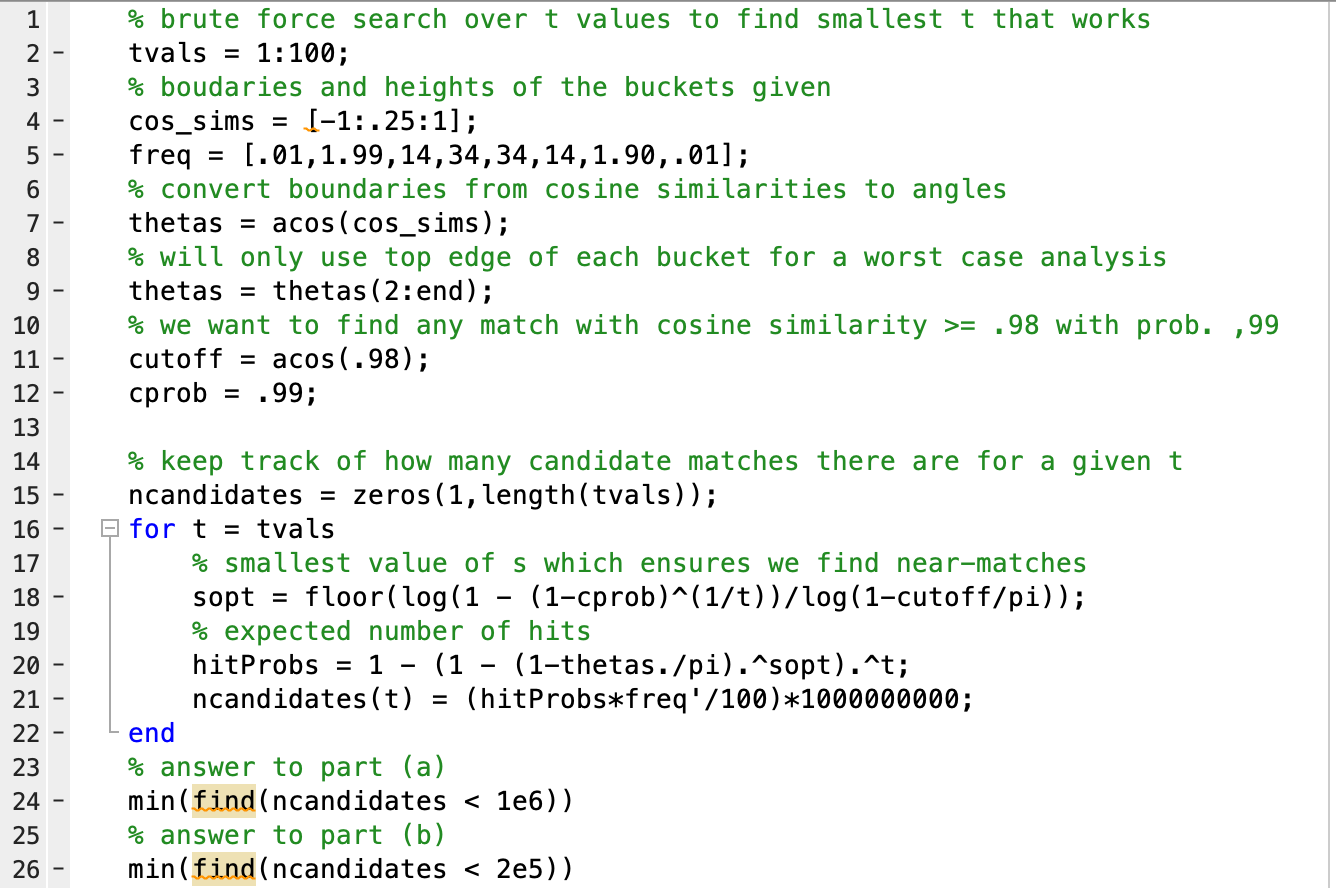
\includegraphics[width=\textwidth]{matlabCode.png}
	\end{figure}
	
% 	\section*{Problem 1}
	
% 	We will solve this problem by bounding $\E[\|\mathbf{s} - \boldsymbol{\mu}\|_2^2]$ and applying Markov's inequality. We have:
% 	\begin{align*}
% 		\|\mathbf{s} - \boldsymbol{\mu}\|_2^2 = \|\frac{1}{k}\sum_{i=1}^k (\bv{x}_i - \bs{\mu})\|_2^2 = \frac{1}{k^2}\sum_{i=1}^k \|\bv{x}_i - \bs{\mu}\|_2^2 + \sum_{i\neq j}(\bv{x}_i - \bs{\mu})^T(\bv{x}_j - \bs{\mu}).
% 	\end{align*}
% 	We want to apply linearity of expectation to the expression above to compute $\E[\|\mathbf{s} - \boldsymbol{\mu}\|_2^2]$. In particular, we are given that
% 	\begin{align*}
% 		\E\left[\sum_{i=1}^k \|\bv{x}_i - \bs{\mu}\|_2^2\right] = k\sigma^2
% 	\end{align*}
% 	and  claim that for all $i \neq j$,
% 	\begin{align*}
% 		\E\left[(\bv{x}_i - \bs{\mu})^T(\bv{x}_j - \bs{\mu})\right] = 0.
% 	\end{align*}
% 	To see why this is the case note that, since $\bv{x}_i$ and $\bv{x}_j$ are independent, 
% 	\begin{align*}
% 		\E\left[(\bv{x}_i - \bs{\mu})^T\E\left[(\bv{x}_j - \bs{\mu})\right]\right] = 		\E\left[(\bv{x}_i - \bs{\mu})^T0\right] = 0.
% 	\end{align*}
% 	So, overall we conclude that:
% 	\begin{align*}
% 		\E\left[\|\mathbf{s} - \boldsymbol{\mu}\|_2^2\right] = \frac{1}{k^2}\E\left[\sum_{i=1}^k \|\bv{x}_i - \bs{\mu}\|_2^2\right] = \frac{1}{k}\sigma^2. 
% 	\end{align*}
% 	Applying Markov's inequality, we have that :
% \begin{align*}
% 	\Pr[\|\mathbf{s} - \boldsymbol{\mu}\|_2^2 \geq \frac{1}{\delta}\frac{1}{k}\sigma^2] \leq \delta.
% \end{align*}
% Plugging in $k = \frac{1}{\delta \epsilon^2}$ and taking square roots on the both sides of the inequality inside the probability yields the bound.


% 	\section*{Problem 2}
% 	We first prove a general result on the strong convexity and smoothness of the sum of two functions.
% 	Consider functions $f(\bv{x})$ and $h(\bv{x})$ that are $\alpha_1$-strongly convex, $\beta_1$ smooth, and  $\alpha_2$-strongly convex, $\beta_2$ smooth, respectively. We have that:
% 	\begin{align*}
% 		\frac{\alpha_1}{2}\|\bv{x} - \bv{y}\|_2^2 \leq f(\bv{y}) - f(\bv{x}) - \nabla f(\bv{x})^T(\bv{y} - \bv{x}) \leq \frac{\beta_2}{2}\|\bv{x} - \bv{y}\|_2^2 \\
% 		\frac{\alpha_2}{2}\|\bv{x} - \bv{y}\|_2^2 \leq h(\bv{y}) - h(\bv{x}) - \nabla h(\bv{x})^T(\bv{y} - \bv{x}) \leq \frac{\beta_2}{2}\|\bv{x} - \bv{y}\|_2^2.
% 	\end{align*}
% 	Adding the inequalities, we have:
% 	\begin{align*}
% 		\frac{\alpha_1 + \alpha_2}{2}\|\bv{x} - \bv{y}\|_2^2 \leq f(\bv{y}) + h(\bv{y}) - (f(\bv{x}) + h(\bv{x})) - (\nabla f(\bv{x}) + \nabla h(\bv{x}) )^T(\bv{y} - \bv{x}) \leq 	\frac{\beta_1 + \beta_2}{2}\|\bv{x} - \bv{y}\|_2^2.
% 	\end{align*}
% 	So, we conclude that the function $g(\bv{x}) = f(\bv{x}) + h(\bv{x})$ is $(\alpha_1 + \alpha_2)$-strongly convex. 

% 	Now, consider the function $h(x) = \lambda \|\bv{x}\|_2^2$. The function has gradient $2\lambda \bv{x}$. So we have that:
% 	\begin{align*}
% 		h(\bv{y}) - h(\bv{x}) - \nabla h(\bv{x})^T(\bv{y} - \bv{x}) &= \lambda\|\bv{y}\|_2^2 - \lambda\|\bv{x}\|_2^2 - 2\lambda \bv{x}^T(\bv{y} - \bv{x})\\
% 		 &= \lambda\|\bv{y}\|_2^2 + \lambda\|\bv{x}\|_2^2 - 2\lambda\bv{x}^T(\bv{y}\\
% 		&= \lambda \|\bv{x} - \bv{y}\|_2^2. 
% 	\end{align*}
% 	In other words, the function is $2\lambda$-strongly convex and $2\lambda$-smooth, so has condition number $1$. We conclude that $g(\bv{x}) = f(\bv{x}) + h(\bv{x})$ is $(\alpha_1 + 2\lambda)$-strongly convex, so is convex. Furthermore, $g$'s condition number is:
% 	\begin{align*}
% 		\frac{\beta_1 + 2\lambda}{\alpha_1 + 2\lambda} \leq \frac{\beta_1 + 2\frac{\beta_1}{\alpha_1}\lambda}{\alpha_1 + 2\lambda} = \frac{\beta_1}{\alpha_1}.
% 	\end{align*}
% 	In the first inequality, we used that $\beta_1/\alpha_1 \geq 1$. 

% 	\section*{Problem 3}
% 	\begin{enumerate}[label=(\alph*)]
% 		\item
% 		Call the separation oracles for $A$ and $B$.  If the element is in both sets, it is in $A \cap B$.  Otherwise, at least one of the oracles returned a separating hyperplane; return either of these. That hyperplane separates $\bv{x}$ from either $A$ or $B$, so clearly separates it from $A \cap B$. 
		
% 		\item
% 		We can check in $O(n)$ time if the point $\bv{x}$ is in the $\ell_1$ ball by adding up the magnitude of it's entries. If the point is outside the $\ell_1$ ball, return the vector $\bv{s} = \text{sign}(\bv{x})$ which has a $1$ in index $i$ if $x_i$ is positive and otherwise has a negative $1$. We have that $\bv{s}^T\bv{x} = \|\bv{x}\|_1 > 1$ since $\bv{x}$ is not in the $\ell_1$ ball. On the other hand, we always that $\bv{s}^T\bv{y} \leq \|\bv{y}\|_1$. Specifically, $\bv{s}^T\bv{y} = \sum_{i=1} \pm 1 \cdot |y_i| \leq \sum_{i=1} |y_i| = \|\bv{y}\|_1$. So, $\bv{s}^T\bv{y} \leq 1$ for all $u$ in $\mathcal{A}$. So $(\bv{s}, 1)$ determines a valid separating hyperplane. And $\bv{s}$ can be computed in $O(n)$ time.
		
% 		\item Let $\bv{y} = \text{Proj}_A(\bv{x})$. If $\bv{y} = \bv{x}$ then we are in the set and don't need to return anything. Otherwise, return $(\bv{a}, \bv{a}^T \bv{x})$ as our separating hyperplane, where $\bv{a} = \bv{x} - \bv{y}$
		
% 		Our goal is to prove that, for all $\bv{z}\in \mathcal{A}$, 
% 		\begin{align*}
% 			\bv{z}^T(\bv{x}-\bv{y}) < \bv{x}^T(\bv{x}-\bv{y})
% 		\end{align*}
		
% 		To do so, first observe that, for any $\bv{z}\in \mathcal{A}$, the angle between the vectors $\bv{x} - \bv{y}$ and $\bv{z} - \bv{y}$ must be greater than or equal to 90 degrees. I.e. that $(\bv{x} - \bv{y})^T(\bv{z} - \bv{y}) \leq 0$. To see that this is the case, draw a triangle between $\bv{x}, \bv{y}, \bv{z}$. If the angle was acute, we could draw a line from $\bv{x}$ that meets the line between $\bv{y}$ and $\bv{z}$ at a 90 degree angle. This line would both be in the convex set (since by definition every point on the line between $\bv{y}$ and $\bv{z}$ is) and also be closer to $\bv{x}$ than $\bv{y}$, contradicting the fact that $\bv{y}$ is $\bv{x}$'s projection on to the set. 

% 		If the angle between $\bv{x} - \bv{y}$ and $\bv{z} - \bv{y}$  is greater than 90 degrees, we have that:
% 		\begin{align*}
% 			(\bv{z}-\bv{y})^T(\bv{x}-\bv{y}) < 0 \leq (\bv{x}-\bv{y})^T(\bv{x}-\bv{y}).
% 		\end{align*}
% 		Adding $\bv{y}^T(\bv{x}-\bv{y})$ to both sides of the inequality proves our goal. I.e., we have
% 	shown that for $\bv{a} = \bv{x} - \bv{y}$, for all $\bv{z}\in \mathcal{A}$, $\bv{a}^T \bv{z}  < \bv{a}^T\bv{x}$ , so we have a valid separating hyperplane.
		
% 		\item
% 		We still choose $\bv{a} = \bv{x} - \bv{y}$ as in the previous subproblem. To prove this is a valid separating hyperplane, it suffices to show that for all $\bv{z}'$ in the $\epsilon$-neighborhood of $\mathcal{A}$, that $\bv{a}^T\bv{z}' < \bv{a}^T \bv{x}$ when $\bv{x}$ is not in the $\epsilon$-neighborhood of $\mathcal{A}$. To prove this, first note that $\bv{z}'$ can always be written as the sum $\bv{z}' = \bv{z} + \bv{w}$ where $\bv{z}$ is a point in $\mathcal{A}$ and $\|\bv{w}\|_2 \leq \epsilon$.  
		
% By the same analysis as above, we have that $(\bv{x}-\bv{y})^T \bv{z} < \bv{x}^T (\bv{x}-\bv{y}) -\|\bv{x}-\bv{y}\|_2^2$. We then bound:
% \begin{align}
% 	(\bv{x}-\bv{y})^T \bv{z}' &= (\bv{x}-\bv{y})^T \bv{z} + (\bv{x}-\bv{y})^T \bv{w}\\
% 	&\leq  \bv{x}^T (\bv{x}-\bv{y}) - \|\bv{x} - \bv{y}\|_2^2 + (\bv{x}-\bv{y})^T \bv{w}\\
% 		&\leq  \bv{x}^T (\bv{x}-\bv{y}) - \|\bv{x} - \bv{y}\|_2^2 + \epsilon \|\bv{x}-\bv{y}\|_2.
% \end{align}
% The last inequality follows from Cauchy-Schwarz. Finally, since $\bv{x}$ is not in the $\epsilon$ neighborhood, $\|\bv{x}-\bv{y}\|_2 > \epsilon$, so  $\|\bv{x} - \bv{y}\|_2^2 > \epsilon \|\bv{x}-\bv{y}\|_2$ and thus we conclude that :
% \begin{align*}
% 	(\bv{x}-\bv{y})^T \bv{z}'  <  \bv{x}^T (\bv{x}-\bv{y})  - 0,
% \end{align*}
% which completes the argument.
% 	\end{enumerate}
	
% \section*{Problem 4}
% We start with basically the same analysis from class, where we showed using convexity that:
% \begin{align*}
% 	f(\bv{x}^{(i)}) - f(\bv{x}^*) \leq \frac{\|\bv{x}^{(i)} - \bv{x}^*\|_2^2 - \|\bv{x}^{(i+1)} - \bv{x}^*\|_2^2}{2\eta} + \frac{\eta \|\nabla f(\bv{x}^{(i)})\|_2^2}{2}. 
% \end{align*}
% See e.g. Slide 50 on Lecture 6. They don't need to reprove this from scratch.

% Now, plug in $\eta = \frac{f(\bv{x}^{(i)}) - f(\bv{x}^{*})}{\|f(\bv{x}^{(i)})\|_2}$. We get: 
% \begin{align*}
% 	f(\bv{x}^{(i)}) - f(\bv{x}^*) \leq \frac{\|\bv{x}^{(i)} - \bv{x}^*\|_2^2 - \|\bv{x}^{(i+1)} - \bv{x}^*\|_2^2}{2(f(\bv{x}^{(i)}) - f(\bv{x}^*))}\cdot\|\nabla f(\bv{x}^{(i)})\|_2^2 + \frac{f(\bv{x}^{(i)}) - f(\bv{x}^*)}{2}. 
% \end{align*}
% Using that $\|\nabla f(\bv{x}^{(i)})\|_2^2 \leq G^2$, we have:
% \begin{align*}
% \frac{f(\bv{x}^{(i)}) - f(\bv{x}^*)}{2}\leq \frac{\|\bv{x}^{(i)} - \bv{x}^*\|_2^2 - \|\bv{x}^{(i+1)} - \bv{x}^*\|_2^2}{2(f(\bv{x}^{(i)}) - f(\bv{x}^*))}\cdot G^2. 
% \end{align*}
% And multiplying through by $2(f(\bv{x}^{(i)}) - f(\bv{x}^*)$, we have:
% \begin{align*}
% 	(f(\bv{x}^{(i)}) - f(\bv{x}^*))^2 \leq \left(\|\bv{x}^{(i)} - \bv{x}^*\|_2^2 - \|\bv{x}^{(i+1)} - \bv{x}^*\|_2^2\right)\cdot G^2
% \end{align*}
% Now we use a telescoping sum argument as before to get that:
% \begin{align*}
% 	\sum_{i=0}^{T-1} (f(\bv{x}^{(i)}) - f(\bv{x}^*))^2 \leq \left(\|\bv{x}^{(0)} - \bv{x}^*\|_2^2 - \|\bv{x}^{(T)} - \bv{x}^*\|_2^2\right)\cdot G^2 \leq \|\bv{x}^{(0)} - \bv{x}^*\|_2^2\cdot G^2 \leq R^2\cdot G^2. 
% \end{align*}
% I.e. 
% \begin{align*}
% 	\frac{1}{T}\sum_{i=0}^{T} (f(\bv{x}^{(i)}) - f(\bv{x}^*))^2 \leq \frac{R^2 G^2}{T}.
% \end{align*}
% This implies that the average squared error is less than or equal to $R^2G^2/T$, so there must be some $i$ such that $(f(\bv{x}^{(i)}) - f(\bv{x}^*))^2 \leq R^2G^2/T$. We conclude that:
% \begin{align*}
% 	f(\hat{\bv{x}}) - f(\bv{x}^*) \leq RG/\sqrt{T}. 
% \end{align*}
% Setting $T = R^2G^2/\epsilon^2$ yields the desired result. 


% \section*{Problem 5}

% 			1. To solve this problem, we show that $\sum_{i=1}^n \|\bv{x}_i\|_2^2 = \frac{1}{2n}\sum_{i,j} \bv{D}_{i,j}$.
% 			\begin{align*}
% 				\sum_{i,j} \bv{D}_{i,j} = \sum_{i} \sum_{j} \|\bv{x}_i\|_2^2 + \|\bv{x}_j\|_2^2 - 2\bv{x}_i^T\bv{x}_j = \sum_{i} \sum_{j} \|\bv{x}_i\|_2^2 + \|\bv{x}_j\|_2^2 - 2\bv{x}_i^T\sum_{j} \bv{x}_j.
% 			\end{align*}
% 			By our assumption that our points are centered around the origin, $\sum_{j} \bv{x}_j = \bv{0}$, so we conclude 
% 			\begin{align*}
% 			\sum_{i,j} \bv{D}_{i,j} = \sum_{i,j} \|\bv{x}_i\|_2^2 + \|\bv{x}_j\|_2^2 = 2n \sum_{i} \|\bv{x}_i\|_2^2.
% 			\end{align*}
% 			2. Similarly, using the same assumption, we can have that for any $i$, 
% 			\begin{align*}
% 			\sum_{j} \bv{D}_{i,j} =\sum_{j} \|\bv{x}_i\|_2^2 + \|\bv{x}_j\|_2^2 - 2\bv{x}_i^T\bv{x}_j = n \|\bv{x}_i\|_2^2 + \sum_j \|\bv{x}_j\|_2^2.
% 			\end{align*}
% 			So we can compute $\|\bv{x}_i\|_2^2$ via the formula $\|\bv{x}_i\|_2^2 = \frac{1}{n}\left(\sum_{j} \bv{D}_{i,j} - \sum_{j} \|\bv{x}_j\|_2^2\right)$. The second term in parenthesis we can compute using Part 1. 
			
% 			3. Using the norms calculated from part (b), we can form the a matrix $\bv{N}$ where;
% 			\begin{align*}
% 			\bv{N}_{i,j} = \|\bv{x}_i\|_2^2 + \|\bv{x}_j\|_2^2.
% 			\end{align*}
% 			Let $\bv{M} = (\bv{N} - \bv{D})/2$. Notice that $\bv{M}$'s entries satisfy $\bv{M}_{i,j} = \bv{x}_i^T\bv{x}_j$. $\bv{M}$'s $i^\text{th}$ diagonal entry equals $\|\bv{x}_i\|_2^2$. So, it suffices to return any $\bv{W} \in \R^{n\times d}$ such that $\bv{W}\bv{W}^T = \bv{M}$. $\bv{W}$'s rows will have the same pairwise distances as the points in $\bv{X}$, and thus solve the problem. 
			
% 			To find such a $\bv{W}$, we can factor $\bv{M}$ using the SVD. Since it is symmetric, we will get a factorization of the form $\bv{V}\bs{\Sigma}\bv{V}^T$. Only $d$ of $\bs{\Sigma}$'s diagonal entries will be nonzero since $\bv{M}$ is rank $d$ (since $\bv{M} = \bv{X}\bv{X}^T$). So we can we can truncate this factorization to get $\bv{V}_d\bs{\Sigma}_d\bv{V}_d^T = \bv{M}$ where $\bv{V}_d \in \R^{n\times d}$ $\bs{\Sigma}_d\in \R^{d\times d}$. Then we return $\bv{W} =\bv{V}_d \sqrt{\bs{\Sigma}_d}$. 

% 		% 4. Don't need to check implmentation, but just check that they got a reasonable answer. 




	

\end{document}